\documentclass[runningheads]{llncs}

\usepackage[utf8]{inputenc}
\usepackage[T1]{fontenc}
\usepackage[english]{babel}
\usepackage{amsmath,amssymb}
\usepackage{graphicx}
\usepackage{booktabs}
\usepackage{multirow}
\usepackage{array}
\usepackage{enumitem}
\usepackage{url}
\usepackage[dvipsnames]{xcolor}
\usepackage{tikz}
\usetikzlibrary{shapes.geometric,arrows.meta,positioning,calc}
\usepackage[colorlinks=true,
            linkcolor=blue!70!black,
            citecolor=blue!70!black,
            urlcolor=blue!60!black]{hyperref}

\graphicspath{{figures/}}

\newcommand{\sirca}{\textsc{SIRCA-RAG}}

\title{Hybrid Corrective RAG for Grounded Generation
on Peruvian Medicinal Plants}

\titlerunning{Hybrid Corrective RAG for Peruvian Medicinal Plants}

\author{Daniel Marron Carcausto \and
Ower Lopez Arela \and
Antonio Arroyo Paz}

\authorrunning{D. Marron Carcausto et al.}

\institute{Universidad Nacional de San Agust\'{i}n de Arequipa, Arequipa, Peru\\
\email{marrondaniel20@gmail.com, olopeza@unsa.edu.pe, aarroyop@unsa.edu.pe}}

\hypersetup{pdfauthor={Daniel Marron Carcausto, Ower Lopez Arela, Antonio Arroyo Paz},
            pdftitle={Hybrid Corrective RAG for Grounded Generation on Peruvian Medicinal Plants},
            pdfkeywords={Retrieval-Augmented Generation, Corrective RAG, Hybrid Retrieval, Ethnobotany, Large Language Models}}

\begin{document}
\sloppy
\maketitle

\begin{abstract}
Pharmacological evidence on Peruvian medicinal plants is fragmented across bibliographic and biodiversity repositories, which makes systematic consultation slow and error-prone. We present \sirca{} (System for Intelligent Retrieval and Corrective Answers), a bilingual (Spanish/English) retrieval-augmented generation system that fuses dense and BM25 retrieval through weighted Reciprocal Rank Fusion, reranks candidates with a cross-encoder, and routes low-confidence retrievals through a Corrective-RAG (CRAG) stage before citation-bearing generation. Our central finding concerns the router's scoring rule: the default within-batch min--max normalization largely suppresses the corrective routes, accepting 20 of 27 out-of-distribution probes and 7 of 10 off-domain queries, whereas a per-document absolute transformation of the reranker logits accepts 8 of 27 and rejects every off-domain query. We call it an \emph{absolute transformation} rather than a \emph{calibration}, since we do not verify that the transformed scores match empirical correctness frequencies. The system indexes 6,481 documents (32,569 chunks, 91 species) selected from 16,486 collected records. On a 50-question bilingual benchmark with author-validated references it reaches an MRR of $0.897$ and an NDCG@10 of $0.887$, and an experimental grounding proxy (Fidelity) reaches $0.670$ over an extended set of 80 queries. The reranker's contribution to Fidelity is directionally consistent but not statistically significant ($p{=}0.082$), and grounded generation is weaker for Spanish than for English queries. Code, index and per-query results are publicly released.

\keywords{Retrieval-Augmented Generation \and Corrective RAG \and Hybrid Retrieval \and Peruvian Ethnobotany \and Large Language Models}
\end{abstract}

\section{Introduction}
\label{sec:intro}

Peru hosts around 25,000 plant species, of which between 1,400 and 5,000 have some documented pharmacological evidence~\cite{bussmann2011toxicity,bussmann2006traditional}. Evidence on a given species, such as \textit{Uncaria tomentosa} or \textit{Croton lechleri}, is nevertheless scattered across PubMed, national biodiversity databases and international records~\cite{gonzales2012ethnobiology,lock2016bioactive}, so assembling a systematic review is slow and prone to gaps.

Large Language Models (LLMs) can summarize large volumes of text, and Retrieval-Augmented Generation (RAG)~\cite{lewis2020retrieval} conditions them on retrieved documents. In the medical domain, however, RAG pipelines frequently retrieve irrelevant passages and produce pharmacological statements that are fluent but unsupported~\cite{gao2024retrieval,ji2023survey}; models trained on biomedical text are not exempt~\cite{gu2021domain,lee2020biobert}. Corrective RAG (CRAG)~\cite{yan2024crag} addresses this by assessing the usefulness of the retrieved evidence before generation and, when it is insufficient, reformulating the query or falling back to web search.

We present \sirca{} (System for Intelligent Retrieval and Corrective Answers), which adapts CRAG to Peruvian medicinal flora through four design decisions: (i)~hybrid retrieval that fuses \texttt{multilingual-e5-base} dense vectors~\cite{wang2024e5} with BM25~\cite{robertson2009bm25} through Reciprocal Rank Fusion (RRF)~\cite{cormack2009rrf}; (ii)~a cross-encoder reranker~\cite{nogueira2019passage}, which captures fine-grained technical distinctions that bi-encoders miss; (iii)~a confidence-based router that, instead of generating from weak evidence, reformulates the query or falls back to a live literature search; and (iv)~a Chain-of-Thought protocol~\cite{wei2022chain} that makes the generator extract, verify and only then compose the answer, citing the supporting passage. The contributions of this work are:
\begin{itemize}[leftmargin=*,itemsep=1pt,topsep=2pt]
  \item a bilingual CRAG architecture for question answering on Peruvian medicinal plants;
  \item a curated corpus of 16,486 collected records, of which 6,481 documents covering 91 species are indexed, and a 50-question bilingual benchmark with author-validated reference answers;
  \item the empirical finding that within-batch score normalization suppresses corrective routing, supported by a head-to-head comparison against a per-document absolute transformation on the same queries;
  \item an evaluation that combines ablations, a generator swap, a per-language analysis and an experimental grounding proxy (Fidelity), with code, index and per-query results publicly released.
\end{itemize}

\section{Related Work}
\label{sec:related}

\textbf{RAG Ecosystem and Corrective Variants.} The paradigm was introduced by Lewis et al.~\cite{lewis2020retrieval}, who showed that conditioning generation on retrieved documents improves answer quality; Gao et al.~\cite{gao2024retrieval} later surveyed the variants that subsequently emerged. Among them, the corrective proposal of Yan et al.~\cite{yan2024crag} is especially relevant to this work, since it evaluates retrieval quality before generation. We adopt this same philosophy, although instead of training a dedicated evaluator we use the \emph{logits} of an already-trained \emph{cross-encoder} directly. Recent empirical evidence supports this design choice: Gangavarapu et al.~\cite{gangavarapu2025corrective} report that corrective RAG consistently improves accuracy over naive retrieval on question-answering benchmarks. Self-RAG~\cite{asai2024selfrag} also allows the LLM to decide when it needs additional information by generating special tokens, but it requires modifying the LLM internally, which exceeds the computational budget of this project.

\textbf{Reliability of Medical RAG.} In the medical domain, retrieval is not universally beneficial. Xie et al.~\cite{xie2026retrievalhurts} show, on MedQA-USMLE, that several RAG configurations underperform a pure-LLM baseline because retrieval injects distractors roughly as often as it supplies missing evidence---a dual effect that motivates confidence-aware routing rather than unconditional retrieval. Wo{\l}k~\cite{wolk2025clinical} likewise frames hallucination mitigation as the central requirement for clinical decision support. These findings justify our emphasis on a strict faithfulness metric and on a corrective router able to abstain when the retrieved evidence is insufficient.

\textbf{Hybrid Search and Reranking.} There is consistent evidence that combining dense and sparse retrieval outperforms either approach alone~\cite{karpukhin2020dense}, as each closes gaps that the other leaves open~\cite{sinha2026lexicalsemantic}. We therefore use RRF~\cite{cormack2009rrf} to combine \texttt{e5-base}~\cite{wang2024e5} with BM25~\cite{robertson2009bm25}, a method that does not require labeled data to calibrate combination weights; we note that Bruch et al.~\cite{bruch2023fusion} show convex-combination fusion can surpass RRF in some settings, a refinement we leave open. Fusion is particularly valuable for the long-tail taxonomic terms that pervade our corpus, where entity-aware hierarchical retrieval yields substantial recall gains~\cite{peng2026hce}. The fused pool is subsequently refined by a \emph{cross-encoder}~\cite{nogueira2019passage}; consistent with our ablation study, Elkiran and Rasheed~\cite{elkiran2026rerankerpairings} identify the retriever--reranker pairing as a key quality--efficiency trade-off in RAG pipelines.

\textbf{Evaluation Methodology.} Our generation metrics follow the definitions of the RAGAs framework~\cite{es2023ragas}, reimplemented with cross-encoder scoring so that no external LLM is needed to compute them, and we complement them with an \emph{LLM-as-judge} cross-check~\cite{zheng2023mtbench} (Sec.~\ref{sec:llm_judge}).

\textbf{Regional, Multilingual and Domain-Specific RAG.} Xiong et al.~\cite{xiong2024mirage}, with their MIRAGE project, showed that RAG outperforms models without retrieval on medical tasks, and Aljohani and Alsanoosy~\cite{aljohani2026hybridmedical} confirm the benefit of hybrid retrieval for medical question answering specifically. Bilingual operation is central to our setting: Chirkova et al.~\cite{chirkova2024multilingual} characterize the components required for a well-performing multilingual RAG pipeline, while low-resource medical deployments---such as medication question answering over Yor\`ub\'a drug labels~\cite{adebesin2026yoruba}---show that hybrid signals are especially useful when data is scarce. For medicinal-plant knowledge specifically, Riddhi et al.~\cite{riddhi2025indianplants} integrate Indian flora through a RAG pipeline, but without corrective routing or a faithfulness-oriented evaluation. In the Latin American context, Monroy Barrios et al.~\cite{monroy2026finetuning} fine-tuned a model on Peruvian flora texts, achieving a substantial reduction in perplexity, although the acquired knowledge remains encapsulated in the model's parameters and is not externally auditable. We favor RAG precisely because it allows the source document of each claim to be traced, an important requirement in the pharmacological domain. As a complementary architecture, Collanqui et al.~\cite{collanqui2026cagrag} contrasted RAG with \emph{Cache-Augmented Generation} over a single institutional regulation; we do not compare against it numerically, since its corpus (one document), domain (administrative), and $k{=}1$ retrieval differ too much from ours (16,486 collected records, 91 indexed species) for an isolated figure to be informative. To the best of our knowledge, no prior work combines a CRAG pipeline with hybrid retrieval applied to Andean medicinal plants.

\section{System Architecture}
\label{sec:architecture}

\sirca{} runs five sequential steps per query, orchestrated in Python with FastAPI and LangGraph (Fig.~\ref{fig:architecture}).

\begin{figure}[!ht]
  \centering
  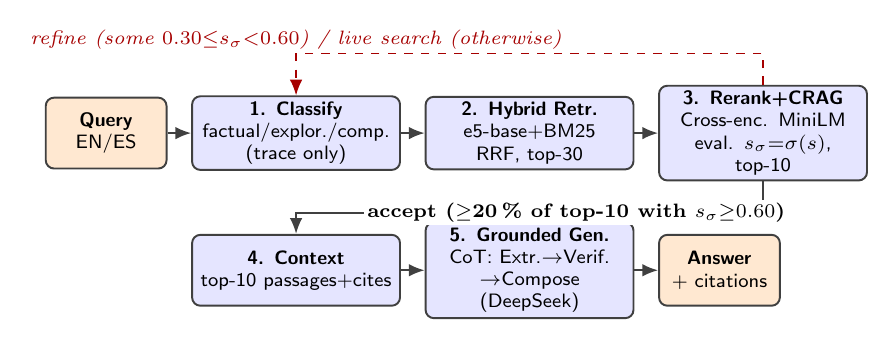
\begin{tikzpicture}[
    font=\sffamily\scriptsize,
    >={Latex[length=2mm,width=1.6mm]},
    phase/.style={rectangle, rounded corners=3pt, draw=black!75, line width=0.7pt,
      minimum height=9mm, text width=25mm, align=center, fill=blue!10, inner sep=2pt},
    io/.style={rectangle, rounded corners=3pt, draw=black!75, line width=0.7pt,
      fill=orange!18, minimum height=9mm, text width=13mm, align=center},
    flow/.style={->, line width=0.7pt, draw=black!75},
    branch/.style={->, line width=0.5pt, draw=red!65!black, dashed},
    blab/.style={font=\scriptsize\itshape, text=red!65!black, fill=white, inner sep=1pt}
  ]
  \node[io] (query) at (0,0) {\textbf{Query}\\{\scriptsize EN/ES}};
  \node[phase, right=3mm of query] (cls)
    {\textbf{1. Classify}\\{\scriptsize factual/explor./comp.}\\{\scriptsize (trace only)}};
  \node[phase, right=3mm of cls] (hyb)
    {\textbf{2. Hybrid Retr.}\\{\scriptsize e5-base+BM25}\\{\scriptsize RRF, top-30}};
  \node[phase, right=3mm of hyb] (crag)
    {\textbf{3. Rerank+CRAG}\\{\scriptsize Cross-enc. MiniLM}\\{\scriptsize eval. $s_{\sigma}{=}\sigma(s)$, top-10}};
  \draw[flow] (query)--(cls); \draw[flow] (cls)--(hyb); \draw[flow] (hyb)--(crag);
  \node[phase, below=8mm of cls.south, anchor=north] (ctx)
    {\textbf{4. Context}\\{\scriptsize top-10 passages+cites}};
  \node[phase, right=3mm of ctx] (gen)
    {\textbf{5. Grounded Gen.}\\{\scriptsize CoT: Extr.$\rightarrow$Verif.}\\{\scriptsize $\rightarrow$Compose (DeepSeek)}};
  \node[io, right=3mm of gen] (ans) {\textbf{Answer}\\{\scriptsize + citations}};
  \draw[flow] (ctx)--(gen); \draw[flow] (gen)--(ans);
  \draw[flow] (crag.south)--++(0,-4mm)-|(ctx.north)
    node[pos=0.2, font=\scriptsize\bfseries, fill=white, inner sep=1pt]{accept ($\geq$20\,\% of top-10 with $s_{\sigma}{\geq}0.60$)};
  \draw[branch] (crag.north)--++(0,4mm)-|(cls.north)
    node[pos=0.5, blab, anchor=south]{refine (some $0.30{\leq}s_{\sigma}{<}0.60$) / live search (otherwise)};
  \end{tikzpicture}
  \caption{\sirca{}'s five-phase pipeline. Classification labels the query (factual/exploratory/comparative) for traceability; hybrid retrieval uses weighted RRF with a fixed $\alpha{=}0.6$ (Eq.~\ref{eq:rrf}); the cross-encoder scores each of the top-10 passages, $s_\sigma$ is the logistic transform of its logit, and the CRAG router decides between accepting the batch and the corrective routes (dashed arrows); generation follows a Chain-of-Thought protocol.}
  \label{fig:architecture}
\end{figure}

The pipeline first labels each query as \textit{factual}, \textit{exploratory} or \textit{comparative} from lexical patterns; the label is recorded in the execution trace for explainability. An earlier version also used it to select a category-specific fusion weight $\alpha$; a held-out $\alpha$ sweep (Sec.~\ref{sec:wilcoxon}) showed that a per-category weight, even when tuned, does not improve on a fixed one, so retrieval always uses $\alpha{=}0.6$.

Retrieval then runs two branches in parallel: \texttt{multilingual-e5-base}~\cite{wang2024e5} embeds the query into a 768-dimensional space searched with FAISS~\cite{johnson2021billion}, and BM25~\cite{robertson2009bm25} matches exact terms that the dense representation may miss. The two ranked lists are merged by a weighted variant of RRF~\cite{cormack2009rrf}. Writing $r_d(q,x)$ and $r_s(q,x)$ for the rank of chunk $x$ under dense and sparse retrieval, counted from $0$, the fused score is
\begin{equation}
\label{eq:rrf}
\mathrm{RRF}_\alpha(q,x) \;=\; \frac{\alpha}{k + r_d(q,x) + 1} \;+\; \frac{1-\alpha}{k + r_s(q,x) + 1},
\end{equation}
with $k{=}60$, $\alpha{=}0.6$, and a term omitted when the chunk is absent from that list. Each branch returns its top 30 chunks. Note that $\alpha$ weights the two \emph{rank-reciprocal} contributions; it is not a convex combination of similarity scores. The top 30 fused chunks form the candidate pool. This parameterization has a consequence we quantify in Sec.~\ref{sec:pool}.

The 30 candidates are reranked by \texttt{ms-marco-MiniLM-L-12-v2}~\cite{nogueira2019passage}, which scores each query--passage pair jointly, and the top 10 are retained. Each retained passage receives the logistic transform of its raw logit, $s_\sigma{=}\sigma(s)$, and the router applies a three-way rule: it \textsc{accept}s the batch when at least $20\,\%$ of the passages reach $s_\sigma{\geq}0.60$; otherwise it triggers \textsc{refine} (query reformulation and re-retrieval, at most twice) when some passage lies in $[0.30,\,0.60)$; and otherwise it takes the \textsc{web\_search} route, a live search of PubMed and Europe PMC for records outside the local index. Sec.~\ref{sec:crag_validation} shows that this per-document transformation, rather than a normalization over the batch, is what makes the corrective routes reachable.

The ten retained passages, with their bibliographic metadata, are passed to DeepSeek V4-Flash~\cite{deepseek2026v4}\footnote{Accessed through the official DeepSeek API (\url{https://api.deepseek.com}), model identifier \texttt{deepseek-v4-flash}.} with a prompt that imposes an extract--verify--compose sequence, requires a citation for every statement, and explicitly forbids content not supported by the passages.

\section{Corpus and Evaluation}
\label{sec:experiments}

\textbf{Corpus.} The corpus was assembled from eight repositories: the bibliographic sources PubMed, Europe PMC, Semantic Scholar and CrossRef, and the structured databases GBIF, PeruNPDB, WFO and COCONUT. We targeted 100 plants from southern Peru and removed duplicate articles by cross-checking DOIs, retaining 16,486 unique records. It is important to separate what was \emph{collected} from what is \emph{retrievable}: only records whose text mentions one of the catalogued species are indexed, which yields the retrieval index actually used in every experiment below --- 6,481 documents split into 32,569 chunks covering 91 species. What is indexed is title plus abstract, not full text (a median of 1,461 characters per document); chunks are 512 \emph{characters} with 64 characters of overlap, which is a median of 51 words. Of the eight repositories, the four bibliographic ones supply every indexed document (PubMed 3,263, Europe PMC 2,016, CrossRef 943 and Semantic Scholar 260 records in the released record list); the four structured databases (GBIF, PeruNPDB, WFO, COCONUT) were queried for taxonomic and phytochemical validation but contribute no indexed chunks, since their records are field-structured rather than prose. Nine of the 100 species have no indexed literature (e.g., \textit{Adesmia spinosissima} and \textit{Berberis lutea}, mostly high-altitude taxa); we keep them deliberately as a stress-test family for the corrective router (Sec.~\ref{sec:crag_validation}). The index embeddings, the per-chunk bibliographic metadata and the list of indexed records are released in the public repository. The abstracts themselves are third-party copyrighted material, so the corpus is released as identifiers that can be re-fetched from their source repositories rather than as redistributed text; re-fetching those records and re-running the indexing script rebuilds the index.

\textbf{Benchmark.} The benchmark comprises 50 questions in Spanish and English (factual, exploratory and comparative) about 12 species, each with a reference answer validated by the authors. The evaluation covers three query sets: the 50 benchmark questions; 30 template queries on 30 additional catalogued species, which test whether retrieval quality degrades outside the verified subset; and a set of out-of-distribution probes designed to exercise the corrective routes.

\textbf{Out-of-distribution probe set.} Alongside the benchmark we use 27 probes,
grouped in three families (Table~\ref{tab:probe_families}). Family~A is not a sample: it
is the complete set of the 9 catalogued species that have no indexed literature, so it is
exhaustive by construction. Families~B and~C are hand-built diagnostic sets that target
the inputs each corrective route is designed for: 10 queries from unrelated technical,
economic and general-interest domains (B), and 8 strings degraded by repetition, noise
characters or missing words (C). They are deliberately \emph{not} a statistical sample of
any population, and we draw no significance claims from them; their purpose is to check
that each route fires on input designed to trigger it. The probes also differ from the
50-query benchmark in what can be measured: they have no author-validated reference
answers, so only the routing decision is scored, never the content of the reply.

\begin{table}[!ht]
\centering
\caption{The three out-of-distribution probe families, with one verbatim example each and
the route the design expects. Family~A is exhaustive (all 9 catalogued species without
indexed literature); B and C are diagnostic sets, not random samples. Only the route is
evaluated, since the probes carry no reference answers.}
\label{tab:probe_families}
\footnotesize
\setlength{\tabcolsep}{4pt}
\begin{tabular}{>{\raggedright\arraybackslash}p{0.25\linewidth} c >{\raggedright\arraybackslash}p{0.40\linewidth} >{\raggedright\arraybackslash}p{0.19\linewidth}}
\toprule
\textbf{Family} & $n$ & \textbf{Example probe (verbatim)} & \textbf{Expected route} \\
\midrule
A. Catalogued species without indexed literature & 9 & \emph{What phytochemical compounds are reported for Adesmia spinosissima?} & \textsc{refine} or \textsc{web\_search} \\
\addlinespace
B. Outside the botanical domain & 10 & \emph{Compare Vue and Svelte for building a modern SPA.} & \textsc{web\_search} \\
\addlinespace
C. Lexically degraded strings & 8 & \emph{medicinal plant peru ??? xxx antioxidant ????} & \textsc{refine} \\
\bottomrule
\end{tabular}
\end{table}

\textbf{Metrics.} Retrieval is evaluated with Context Precision, Context Recall, MRR and NDCG, and generation with BERTScore F1~\cite{zhang2020bertscore}, Semantic Similarity, Entity Coverage (fraction of reference entities named in the answer) and Answer Relevancy~\cite{es2023ragas}. To detect unsupported pharmacological claims we also define \emph{Fidelity}, an experimental grounding proxy that combines a sentence-level cross-encoder support score ($65\,\%$) with content-word overlap against the retrieved context ($35\,\%$); Sec.~\ref{sec:fidelity_weight} examines its sensitivity to this weighting. Component contributions are isolated by ablation, removing one component at a time.

\section{Results}
\label{sec:results}

On the 50-query, 12-species human-verified benchmark, \sirca{} achieves a Context Recall of $0.485$, an MRR of $0.897$ and an NDCG@10 of $0.887$; Fidelity, which is computed over the wider $n{=}80$ set, is $0.670$ (Table~\ref{tab:full_results}, \texttt{full} column). The MRR indicates that, for the large majority of queries, the most relevant document lands in the first or second rank position. No numerical comparison with prior work is attempted, for the reasons given in Sec.~\ref{sec:related}.

On generation, the system attains a BERTScore F1 of $0.820$ (\texttt{roberta-large}), a Semantic Similarity of $0.770$ and an Answer Relevancy of $0.999$. The lowest value is Entity Coverage ($0.428$). Manual inspection of the lowest-scoring answers shows that the generator tends to name only the best-supported compound or species in each statement and omits secondary entities present in the reference, which entity-exhaustive metrics penalize even when the answer is correct. The $35\,\%$ lexical term of Fidelity deliberately penalizes paraphrase of chemical and taxonomic names, where a paraphrase can alter the pharmacological meaning. On the 50-query subset used for the generator comparison, where the two components were measured separately, DeepSeek scores $0.613$ semantic and $0.587$ lexical, which combine to the $0.604$ reported in Table~\ref{tab:multi_llm} (Sec.~\ref{sec:fidelity_weight}).

\begin{table}[!ht]
\centering
\caption{Retrieval metrics of the full pipeline (weighted RRF followed by cross-encoder reranking) on the 12 human-verified species (50 benchmark queries) and on 30 additional catalogued species (30 template queries). $n_{\text{spp}}$ is the number of species and $n_{\text{q}}$ the number of queries. C.\ Prec.\ and C.\ Recall are Context Precision and Context Recall.}
\label{tab:extended_retrieval}
\footnotesize
\setlength{\tabcolsep}{2.5pt}
\begin{tabular}{l c c c c c c c}
\toprule
\textbf{Subset} & $n_{\text{spp}}$ & $n_{\text{q}}$ & \textbf{MRR} & \textbf{NDCG@5} & \textbf{NDCG@10} & \textbf{C.\ Prec.} & \textbf{C.\ Recall} \\
\midrule
Verified & 12 & 50 & $0.897$ & $0.881$ & $0.887$ & $0.430$ & $0.485$ \\
Additional & 30 & 30 & $0.883$ & $0.868$ & $0.867$ & $0.451$ & $0.489$ \\
\bottomrule
\end{tabular}
\end{table}

\textbf{Retrieval generalization.} Table~\ref{tab:extended_retrieval} shows that retrieval quality is preserved when the evaluation is widened from the 12 human-verified species to 30 further species sampled from the catalogue: MRR moves from $0.897$ to $0.883$, NDCG@10 from $0.887$ to $0.867$ and Context Recall from $0.485$ to $0.489$, and no metric changes by more than $0.021$. The retrieval engine is therefore not overfit to the verified subset. We do \emph{not} describe these as \emph{unseen} species: all of them are represented in the index, so the experiment measures performance on species absent from the initial benchmark, not generalization to material outside the corpus.

The remainder of this section reports, in order, the central routing result (Sec.~\ref{sec:crag_validation}), the ablation and its statistical tests (Secs.~\ref{sec:ablation}--\ref{sec:wilcoxon}), the contribution of hybrid fusion (Sec.~\ref{sec:pool}), the generator swap (Sec.~\ref{sec:multi_llm}), the validity of the Fidelity proxy (Secs.~\ref{sec:fidelity_weight}--\ref{sec:llm_judge}) and the per-language analysis (Sec.~\ref{sec:language}).

\subsection{Corrective Routing and Score Normalization}
\label{sec:crag_validation}

The first implementation of the evaluator rescaled the reranker scores of each retrieved batch to $[0,1]$ by min--max normalization. This makes the decision relative to the batch: the best passage of every query is mapped to $1.0$ regardless of its absolute relevance, so the accept branch can be reached even when no retrieved passage is relevant. We replaced it with the per-document logistic transformation $s_\sigma{=}\sigma(s)$ described in Sec.~\ref{sec:architecture}, which does not depend on the other passages retrieved for the same query. We deliberately avoid the term \emph{calibration}: a calibrated score would have to match empirical correctness frequencies, which we do not verify here.

The 27 out-of-distribution probes (Sec.~\ref{sec:experiments}, Table~\ref{tab:probe_families}) test whether the corrective routes fire on the inputs they exist for; they evaluate route selection, not the quality of any subsequent web-supported answer (Limitation~\ref{lim:websearch}). Table~\ref{tab:norm_compare} and Fig.~\ref{fig:crag_routing} compare both scoring rules on the same probes and on the 50 benchmark queries, using one retrieval pass per query, one vector of raw cross-encoder logits and two decision functions.

\begin{figure}[!ht]
\centering
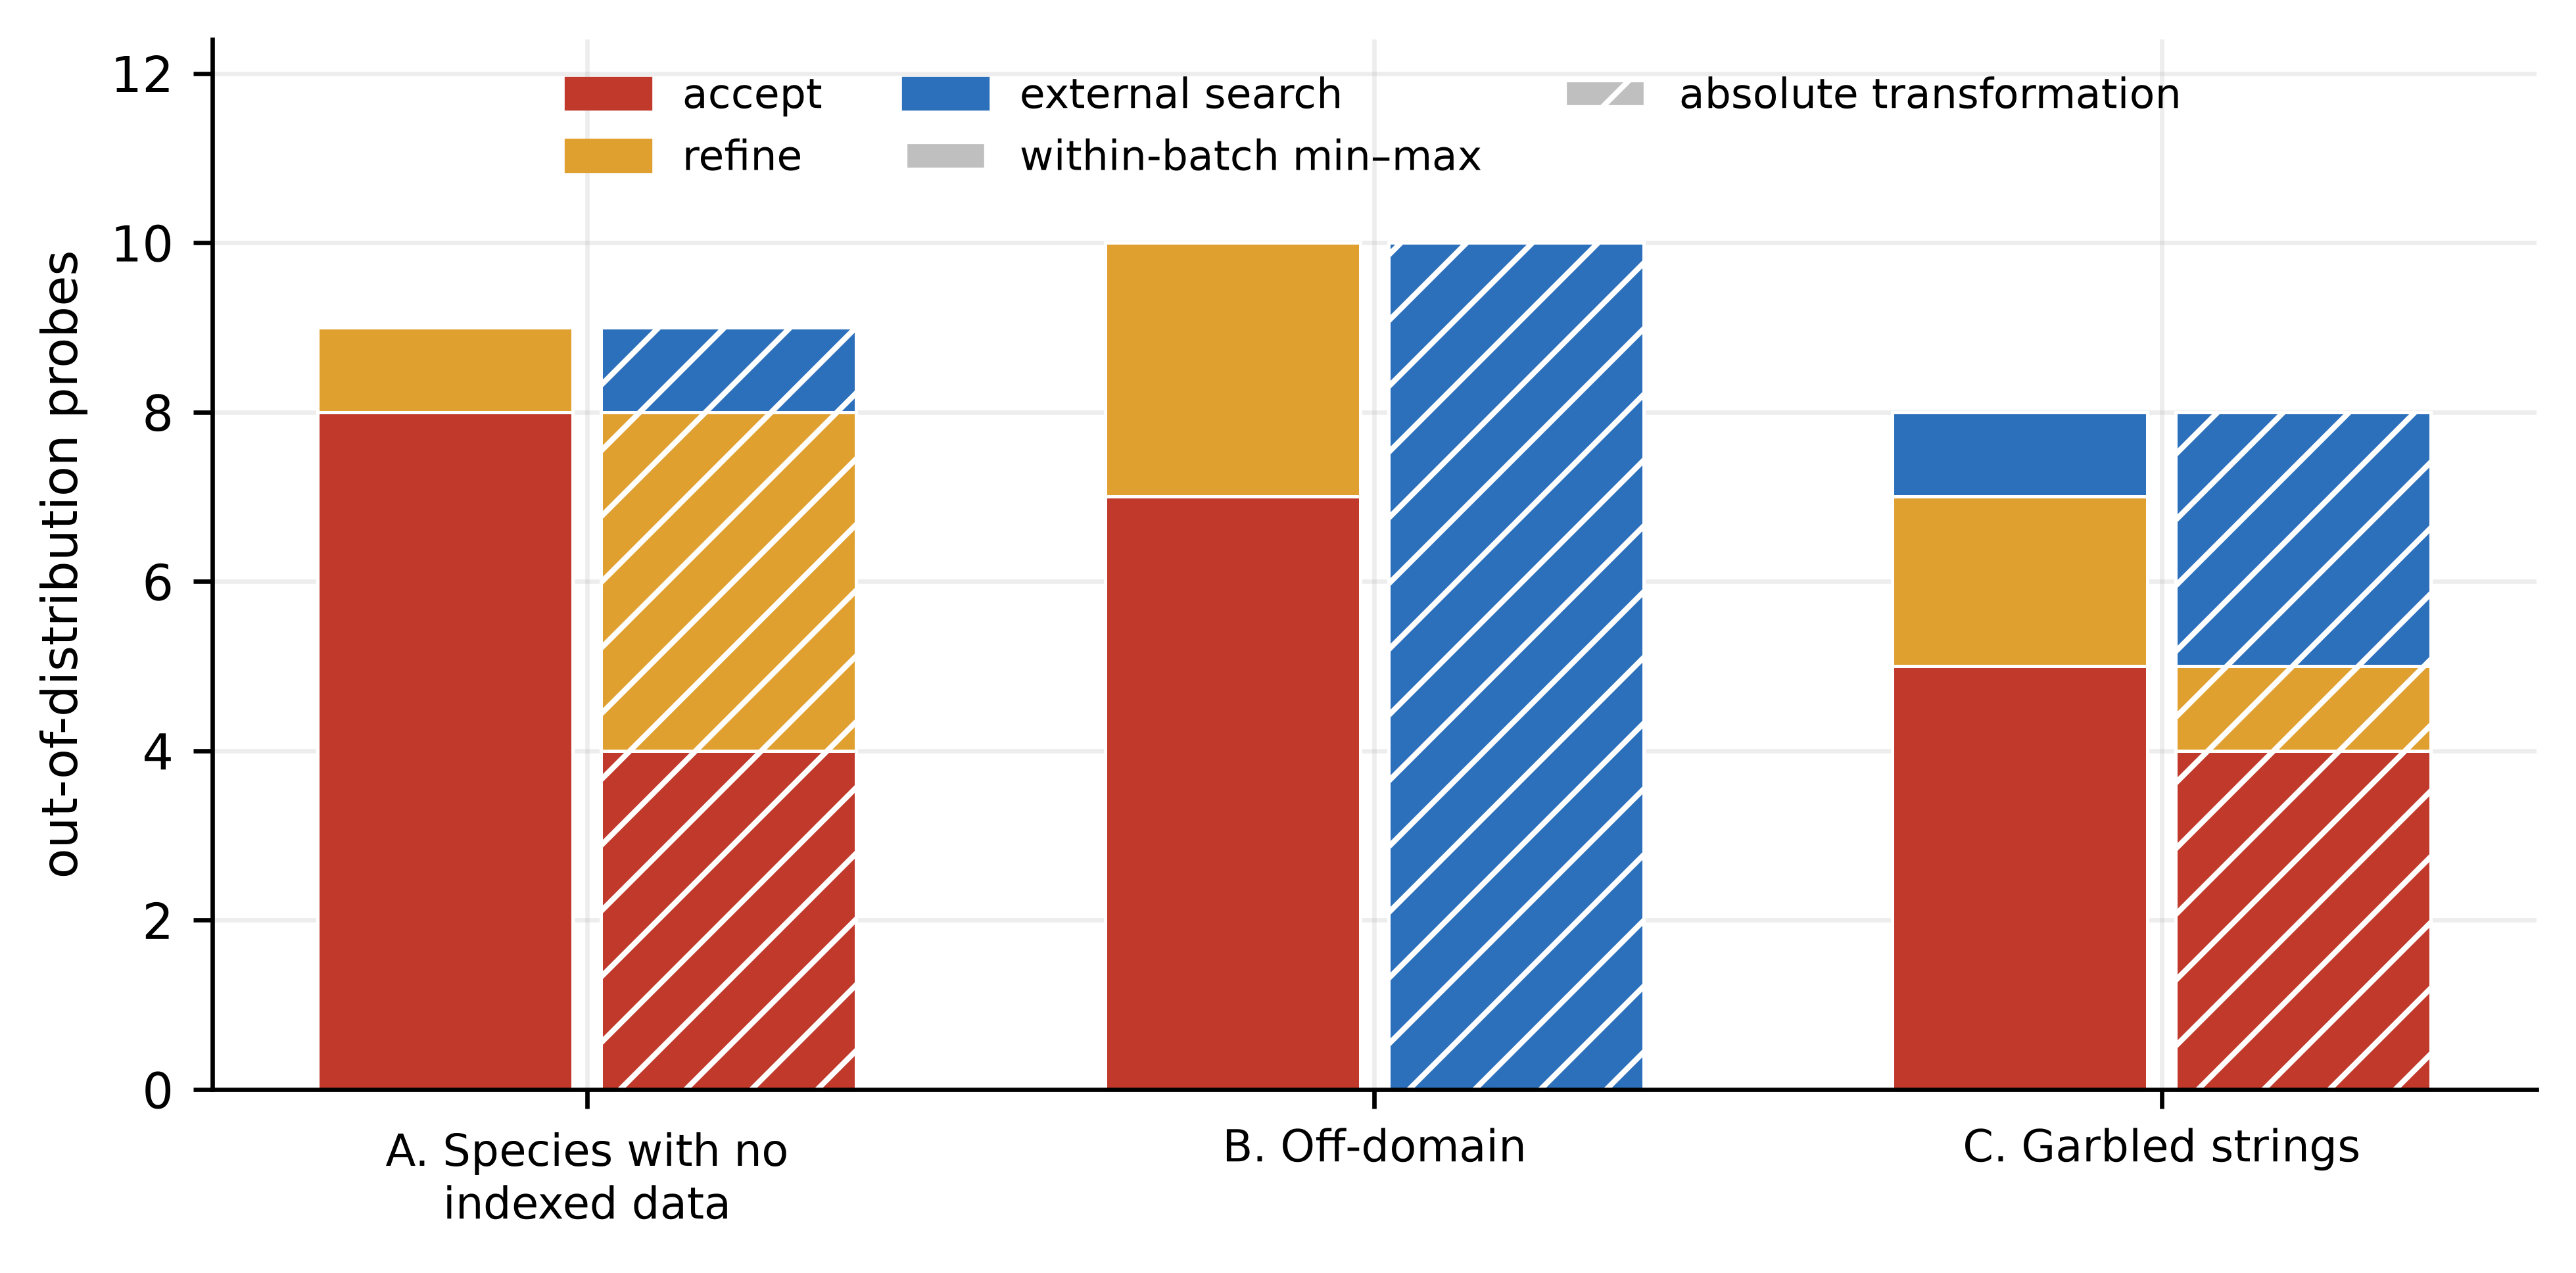
\includegraphics[width=0.85\linewidth]{crag_routing.png}
\caption{Routing of the 27 out-of-distribution probes under the two scoring rules. For each family, the solid bar is the within-batch \textsc{min--max} rule and the hatched bar the per-document absolute transformation; colors give the route taken. Family sizes: A $n{=}9$, B $n{=}10$, C $n{=}8$. The absolute transformation lowers acceptance from $20/27$ to $8/27$ probes and rejects every off-domain query ($0/10$ accepted, vs.\ $7/10$ under \textsc{min--max}).}
\label{fig:crag_routing}
\end{figure}

\begin{table}[!ht]
\centering
\caption{Head-to-head comparison of the two scoring rules on the \emph{same}
27 probes and the \emph{same} 50 benchmark queries. \textsc{min--max} is the
original within-batch implementation, recovered verbatim from the pre-fix revision of
the evaluator; \textsc{sigmoid} is the per-document absolute transformation. The
downstream decision rule (Sec.~\ref{sec:architecture}) is identical in both arms.
\textsc{corrective} counts \textsc{refine} plus \textsc{web\_search}; under \textsc{sigmoid}
the 50 benchmark queries split into 43 \textsc{accept}, 2 \textsc{refine} and 5
\textsc{web\_search}. Boldface marks the intended behavior on off-domain input.}
\label{tab:norm_compare}
\footnotesize
\begin{tabular}{l c c c c c c}
\toprule
 & & \multicolumn{2}{c}{\textsc{min--max} (within-batch)} & \multicolumn{2}{c}{\textsc{sigmoid} (absolute)} \\
\cmidrule(lr){3-4}\cmidrule(lr){5-6}
\textbf{Query set} & $n$ & \textsc{accept} & \textsc{corrective} & \textsc{accept} & \textsc{corrective} \\
\midrule
A. Species with no indexed data &  9 & 8 & 1 & 4 & 5 \\
B. Off-domain                   & 10 & 7 & 3 & \textbf{0} & \textbf{10} \\
C. Garbled strings              &  8 & 5 & 3 & 4 & 4 \\
\midrule
All probes                      & 27 & 20 & 7 & \textbf{8} & \textbf{19} \\
In-domain benchmark             & 50 & 46 & 4 & 43 & 7 \\
\bottomrule
\end{tabular}
\end{table}

Table~\ref{tab:norm_compare} quantifies the defect against its replacement. Within-batch
normalization accepts $20$ of the $27$ out-of-distribution probes ($74\,\%$) vs.\ $8$
($30\,\%$) under the absolute transformation, and accepts $7$ of the $10$ off-domain
queries that the absolute transformation routes to external search without exception
($10/10$). One qualification is required: within-batch normalization does not suppress
the corrective routes altogether. It still triggers $7$ of them across the 27 probes,
since the decision rule also requires at least $20\,\%$ of the batch above threshold,
and min--max sends the worst document of every batch to $0$. The effect is therefore
quantitative: the within-batch rule multiplies the out-of-distribution acceptance rate by
about 2.5 and removes the categorical rejection of off-domain input, without disabling
the corrective routes entirely.

\begin{table}[!ht]
\centering
\caption{Accept rate under the absolute transformation as a function of the accept
threshold (refine threshold fixed at $0.30$), recomputed from the stored raw logits of
the same queries. The desired behavior is a high rate on the in-domain benchmark and a
low one on the probe families; Family C (not shown) is constant at $50\,\%$. Boldface
marks the operating point.}
\label{tab:threshold_sweep}
\footnotesize
\begin{tabular}{l c c c c c c}
\toprule
\textbf{Accept threshold} & $0.30$ & $0.40$ & $0.50$ & $\mathbf{0.60}$ & $0.70$ & $0.90$ \\
\midrule
In-domain benchmark ($n{=}50$)      & $90\,\%$ & $90\,\%$ & $88\,\%$ & $\mathbf{86\,\%}$ & $86\,\%$ & $76\,\%$ \\
Species with no data ($n{=}9$)      & $78\,\%$ & $56\,\%$ & $56\,\%$ & $\mathbf{44\,\%}$ & $44\,\%$ & $22\,\%$ \\
Off-domain ($n{=}10$)               & $0\,\%$  & $0\,\%$  & $0\,\%$  & $\mathbf{0\,\%}$  & $0\,\%$  & $0\,\%$ \\
\bottomrule
\end{tabular}
\end{table}

The thresholds were fixed a priori rather than tuned on the probes, and then checked
for sensitivity (Table~\ref{tab:threshold_sweep}). Off-domain queries never reach \textsc{accept} at any threshold, so they do
not constrain the choice at all; acceptance of no-data species falls in steps from
$78\,\%$ to $22\,\%$ but is flat at $44\,\%$ across every threshold in
$[0.55,\,0.85]$; and in-domain acceptance declines smoothly from $90\,\%$ to
$76\,\%$. The operating point therefore sits on a plateau rather than at an optimum:
every threshold in $[0.55,\,0.85]$ routes both probe families identically, and
$0.60$ is a defensible but not a distinguished choice (Limitation~\ref{lim:thresholds}).

Under the absolute transformation, off-domain queries are routed to external search in $10$ of $10$ cases. For taxa absent from the index, $5$ of $9$ probes trigger a reformulation or the external fallback, while $4$ are accepted because the index supplies context from related taxa of the same genus or family. The router thus rejects out-of-domain input categorically, but it does not distinguish a species without literature of its own from one whose close relatives are well documented. On the 50 benchmark queries, $7$ corrective activations occur ($2$ \textsc{refine}, $5$ \textsc{web\_search}); $5$ of them fall on \textit{exploratory} or \textit{comparative} queries (vs.\ $25$ of the $43$ accepted queries), categories that call for synthesis across sources; with seven activations we report this as a tendency only. In such cases, declaring uncertainty is preferable to producing an unsupported answer. Overall, the per-document absolute transformation makes the corrective routes reachable on out-of-distribution input and on low-confidence in-domain queries, which the batch-relative rule largely prevented (Table~\ref{tab:norm_compare}).

\subsection{Findings from the Ablation}
\label{sec:ablation}

\begin{table}[!ht]
\centering
\caption{Ablation of five configurations. \textbf{Sample sizes differ by column}: the four retrieval metrics are computed over the 50 benchmark queries, while Fidelity is computed over $n{=}80$ (the 50 benchmark queries plus 30 template queries on additional species) with the DeepSeek generator. $\Delta$ is the relative change in Fidelity with respect to \texttt{full}. Boldface marks the best and underlining the worst value per column; no Fidelity difference is statistically significant (Sec.~\ref{sec:ablation}). $^\dagger$\texttt{dense\_only} matches \texttt{full} on every retrieval metric because its Top-10 is identical on all 50 queries; Sec.~\ref{sec:pool} shows this follows from the fusion parameters rather than from the reranker dominating.}
\label{tab:full_results}
\footnotesize
\begin{tabular}{l c c c c c c}
\toprule
\textbf{Config.} & \multicolumn{4}{c}{\textbf{Retrieval} ($n{=}50$)} & \multicolumn{2}{c}{\textbf{Fidelity} ($n{=}80$)} \\
\cmidrule(lr){2-5}\cmidrule(lr){6-7}
 & \textbf{C.Prec.} & \textbf{C.Recall} & \textbf{MRR} & \textbf{NDCG@10} & \textbf{Fidel.} & $\boldsymbol{\Delta}$ \\
\midrule
\texttt{full} & \underline{$0.430$} & $0.485$ & $0.897$ & $0.887$ & $0.670$ & --- \\
\texttt{dense\_only$^\dagger$} & \underline{$0.430$} & $0.485$ & $0.897$ & $0.887$ & $\mathbf{0.677}$ & $+1.1\%$ \\
\texttt{sparse\_only} & $\mathbf{0.465}$ & $\mathbf{0.525}$ & \underline{$0.867$} & \underline{$0.832$} & $0.657$ & $-1.9\%$ \\
\texttt{no\_reranker} & $0.440$ & \underline{$0.484$} & $\mathbf{0.955}$ & $\mathbf{0.900}$ & \underline{$0.640$} & $-4.5\%$ \\
\texttt{no\_crag} & $0.432$ & $0.488$ & $0.897$ & $0.891$ & $0.676$ & $+0.9\%$ \\
\bottomrule
\end{tabular}
\end{table}

\begin{figure}[!ht]
\centering
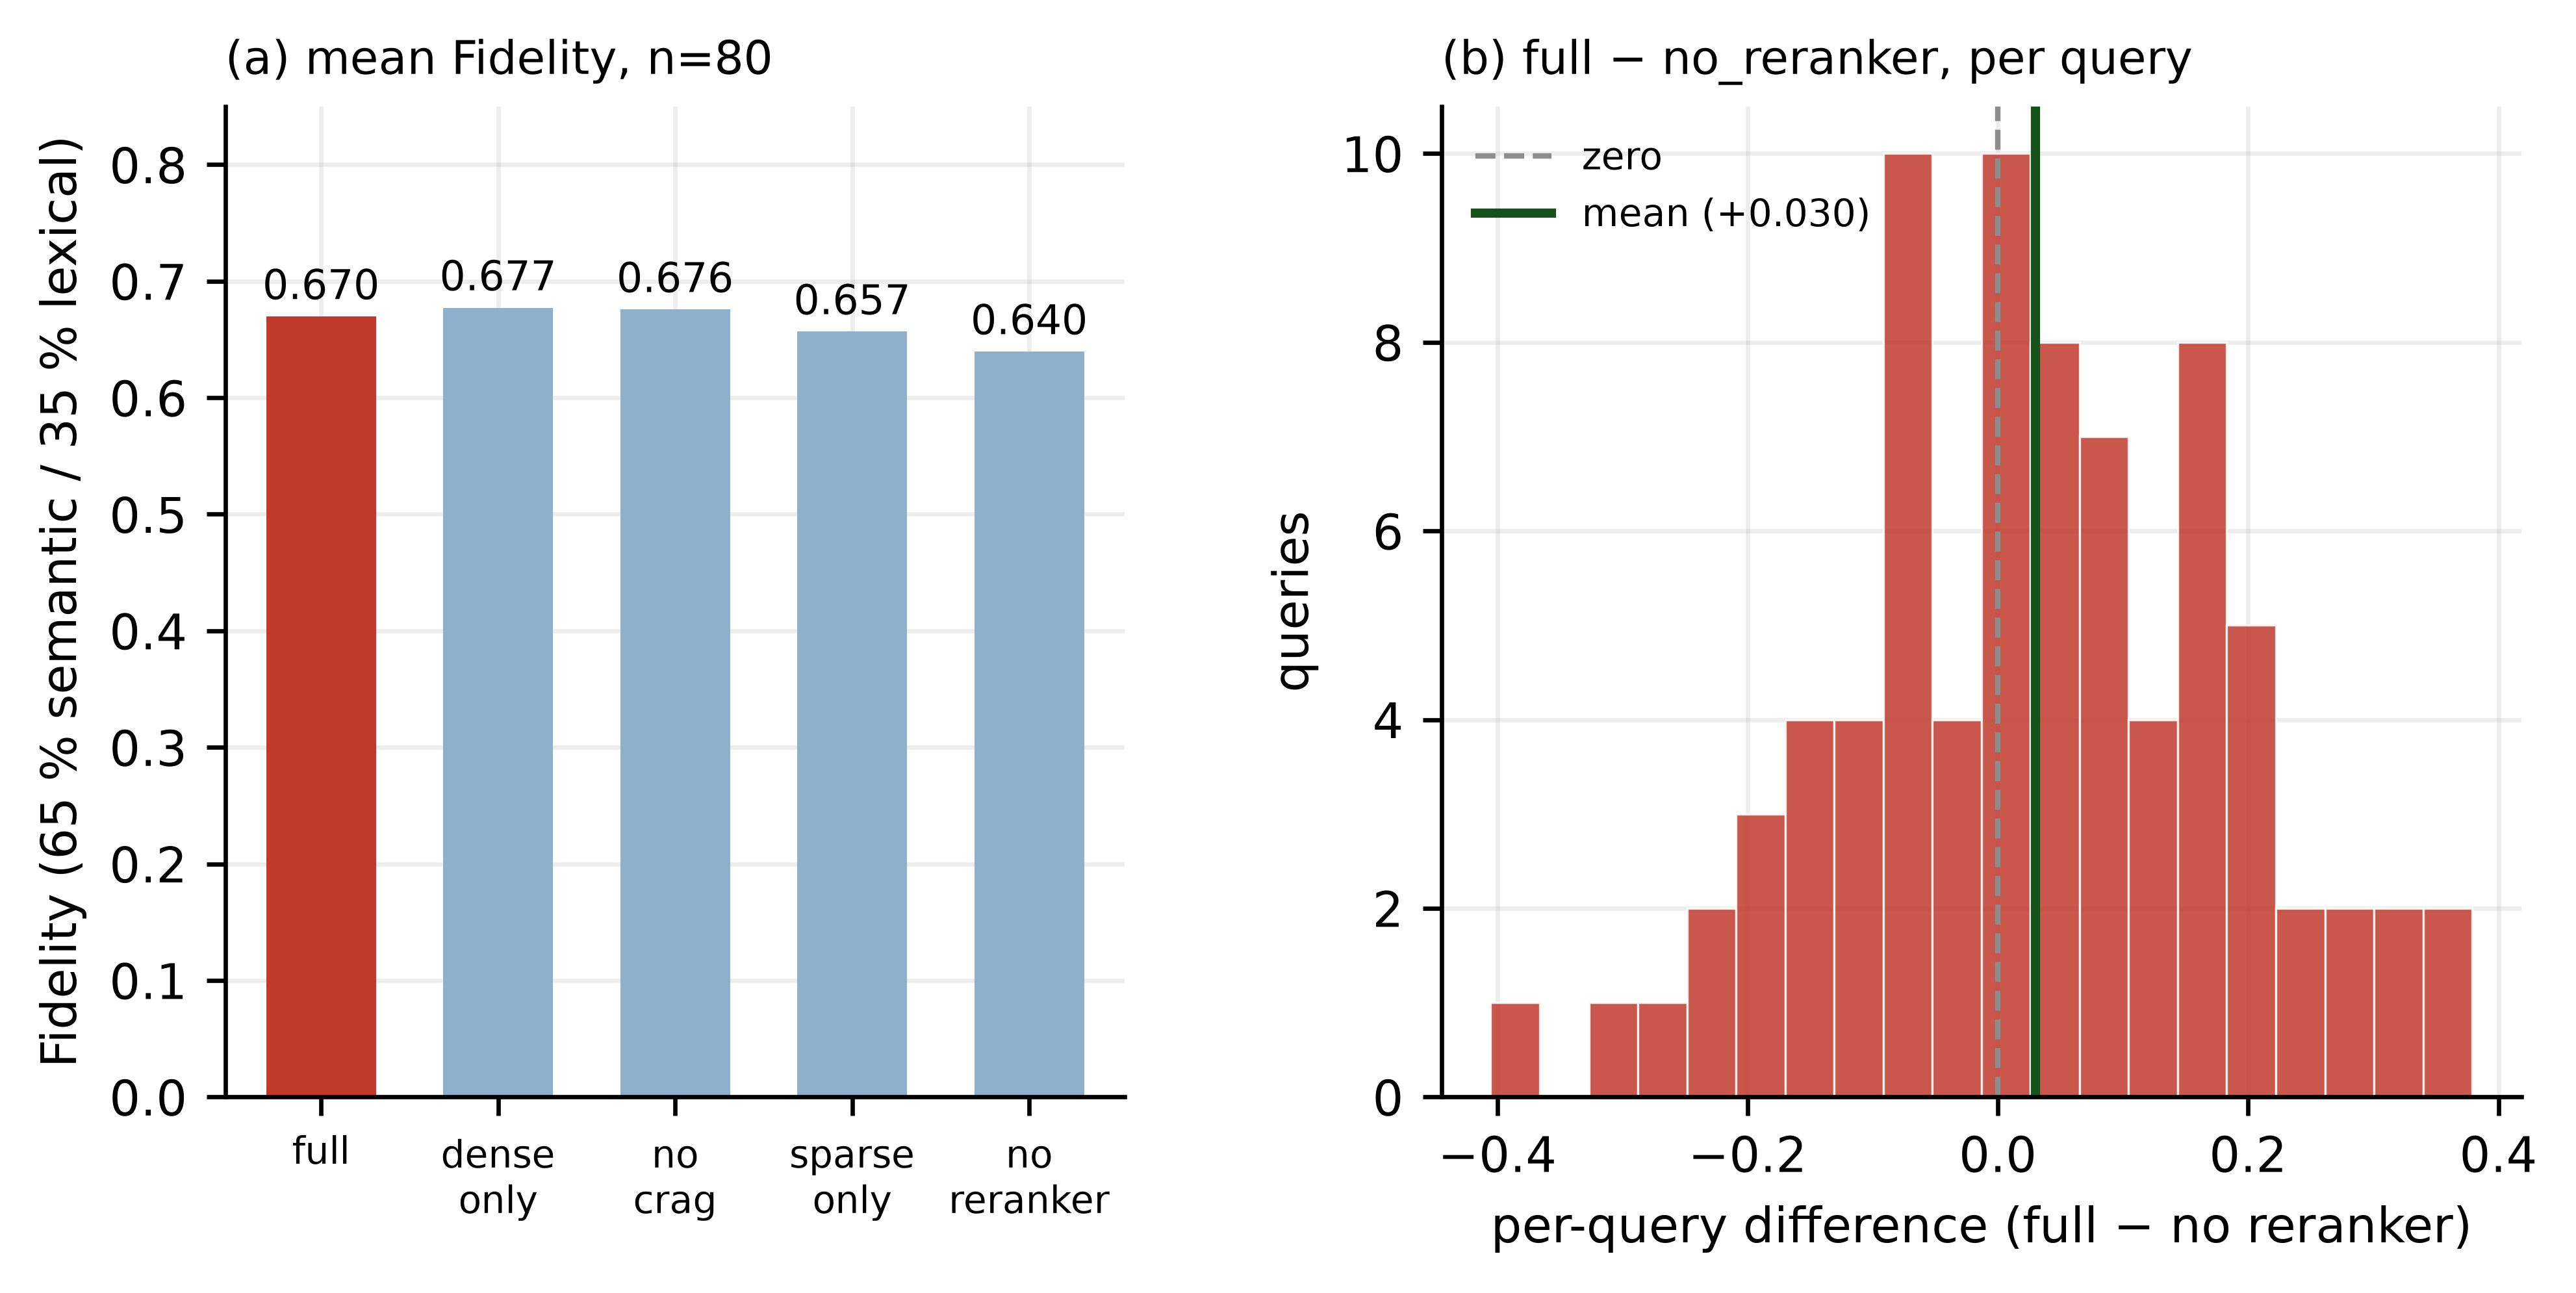
\includegraphics[width=0.92\linewidth]{ablation_fidelity.png}
\caption{Fidelity across the ablation ($n{=}80$ queries, DeepSeek generator). \textbf{(a)}~Mean Fidelity of the five configurations, from $0.640$ (\texttt{no\_reranker}) to $0.677$ (\texttt{dense\_only}); no pairwise difference with \texttt{full} is significant. \textbf{(b)}~Distribution of the per-query difference \texttt{full}~$-$~\texttt{no\_reranker}; the dashed line marks zero and the solid line the mean ($+0.030$). $49$ of the $80$ queries favor \texttt{full}, but the paired Wilcoxon test is not significant two-sided ($p{=}0.082$; one-sided $p{=}0.041$).}
\label{fig:ablation_fidelity}
\end{figure}

Table~\ref{tab:full_results} and Fig.~\ref{fig:ablation_fidelity} yield three observations. \textbf{First}, the cross-encoder is the component most consistently associated with Fidelity. Removing it lowers Fidelity by $4.5\,\%$ relative ($0.670 \rightarrow 0.640$), the largest movement in the column, but the paired Wilcoxon test does not reach two-sided significance ($p{=}0.082$; one-sided $p{=}0.041$; $n{=}80$), and $49$ of the $80$ queries favor \texttt{full}. The other configurations bracket \texttt{full} without significant differences (\texttt{dense\_only} $0.677$, $p{=}0.680$; \texttt{no\_crag} $0.676$, $p{=}0.996$; \texttt{sparse\_only} $0.657$, $p{=}0.412$). The \texttt{dense\_only} row also provides an empirical noise floor: it feeds the generator exactly the same Top-10 as \texttt{full}, so its difference from \texttt{full} ($+0.008$) is pure generation stochasticity. The reranker effect ($-0.030$) is about four times this floor, which explains why its direction is stable across runs while its two-sided significance is not (Limitation~\ref{lim:reranker}). We therefore report it as a consistent directional signal, not as a statistically confirmed effect. \textbf{Second}, \texttt{sparse\_only} attains the best Context Precision ($0.465$) and Recall ($0.525$) but the worst MRR ($0.867$) and NDCG@10 ($0.832$): BM25 alone admits more relevant passages into the pool but orders them worse. \textbf{Third}, \texttt{dense\_only} returns the same Top-10 as \texttt{full} on all 50 queries, which Sec.~\ref{sec:pool} shows to follow from the fusion parameters.

\subsection{Statistical Significance of the Ablation Deltas}
\label{sec:wilcoxon}

Per-query paired Wilcoxon signed-rank tests (two-sided, $n{=}50$) compare each ablation variant with \texttt{full} on the four retrieval metrics (Table~\ref{tab:wilcoxon}). No correction for multiple comparisons is applied: only the Fidelity comparison between \texttt{full} and \texttt{no\_reranker} is interpreted confirmatorily, and the retrieval tests are exploratory.

\begin{table}[!ht]
\centering
\caption{Wilcoxon signed-rank $p$-values (two-sided) against \texttt{full} on per-query retrieval metrics ($n{=}50$), same methodology as Table~\ref{tab:full_results}. $n_{\neq}$ is the number of queries with a non-zero difference on C.Recall; ``---'' marks a configuration whose Top-10 is identical to \texttt{full} ($n_{\neq}{=}0$). \textbf{No value reaches $\alpha{=}0.05$.} The central Fidelity comparison (\texttt{full} vs.\ \texttt{no\_reranker}, $n{=}80$) is reported in the text below.}
\label{tab:wilcoxon}
\footnotesize
\begin{tabular}{l c c c c c}
\toprule
\textbf{Config.} & \textbf{$n_{\neq}$} & \textbf{C.Prec.} & \textbf{C.Recall} & \textbf{MRR} & \textbf{NDCG@10} \\
\midrule
\texttt{dense\_only}    &  0 & --- & --- & --- & --- \\
\texttt{sparse\_only} & 38 & 0.393 & 0.331 & 0.325 & 0.062 \\
\texttt{no\_reranker} & 11 & 0.687 & 0.721 & 0.128 & 0.653 \\
\texttt{no\_crag} &  1 & 0.317 & 0.317 & --- & 0.317 \\
\bottomrule
\end{tabular}
\end{table}

No configuration differs significantly from \texttt{full} at the retrieval level. \texttt{sparse\_only} does not reach significance despite its higher aggregate precision (C.\ Prec.\ $p{=}0.393$; C.\ Recall $p{=}0.331$, $n_{\neq}{=}38$): BM25 alone wins on some queries and loses on others. \texttt{no\_reranker} is not significant on any metric ($p{\geq}0.128$), and \texttt{no\_crag} differs from \texttt{full} on a single query ($p{=}0.317$), where disabling the router changes the final context. \texttt{dense\_only} is identical to \texttt{full} on every query (Sec.~\ref{sec:pool}). An $\alpha$ sweep over 30 held-out species, not used for any reported number, confirmed this invariance: neither a different fixed $\alpha$ nor a tuned per-category $\alpha$ improved on $\alpha{=}0.6$ when evaluated once on the 50 benchmark queries, which motivated removing the per-category weighting (Sec.~\ref{sec:architecture}).

The confirmatory test on Fidelity (\texttt{full} vs.\ \texttt{no\_reranker}, $n{=}80$) gives $p{=}0.082$ two-sided and $p{=}0.041$ one-sided on the final index. It was repeated six times during development as defects were fixed and the index was rebuilt; the direction was the same in all six runs, whereas two-sided significance was reached in three (Limitation~\ref{lim:reranker}). We adopt the final run as the reference. Finally, DeepSeek's Fidelity differs between Table~\ref{tab:multi_llm} ($0.604$) and Table~\ref{tab:full_results} ($0.670$) because the two come from different runs over different query sets (50 vs.\ 80 queries); only within-run comparisons are interpreted.

\subsection{Where Hybrid Fusion Contributes}
\label{sec:pool}

Because \texttt{dense\_only} and \texttt{full} return an identical Top-10 on every query
(Table~\ref{tab:wilcoxon}), the reported benchmark cannot establish an incremental
benefit of hybrid retrieval after reranking. The cause is arithmetic rather than
empirical, and follows from Eq.~\ref{eq:rrf}. With $k{=}60$, 30 candidates per branch and
$\alpha{=}0.6$, the last dense document (rank 29) scores at least $0.6/(60{+}29{+}1)=0.006667$,
while a document found only by BM25 scores at most $0.4/(60{+}0{+}1)=0.006557$. The former is
larger, so \emph{no} document unique to BM25 can enter the pool while 30 dense
candidates exist: we confirmed $0$ such documents across all queries in both indices.
The crossing point is $\alpha^\ast = (k{+}30)/(2k{+}31) = 0.5960$; below it BM25
contributes documents, above it only ranking evidence through the agreement bonus.

Measuring the configurations on the candidate pool \emph{before} the cross-encoder makes
the contribution visible (Table~\ref{tab:pool}). Hybrid fusion improves ranking over
dense-only (NDCG@10 $0.799 \rightarrow 0.824$; C.\ Precision $0.540 \rightarrow
0.553$) while Recall@30 is identical by the argument above. The claim is therefore
narrow: at $\alpha{=}0.6$ the lexical branch re-ranks the dense pool and does not
extend it, and the benefit does not survive the cross-encoder. Lowering $\alpha$ below $0.5960$, or fusing before truncation, is the
experiment that would let the lexical branch contribute coverage; we leave it open.

\begin{table}[!ht]
\centering
\caption{Retrieval metrics on the top-30 candidate pool, before cross-encoder
reranking, on the final index (32,569 chunks). Ground truth is species matching over the union of
dense@30 and sparse@30, so it does not depend on the configuration being scored; 47 of
the 50 queries declare a relevant species. Recall@30 is identical for dense-only and
hybrid because, at $\alpha{=}0.6$, no BM25-unique document enters the pool.}
\label{tab:pool}
\footnotesize
\begin{tabular}{l c c c c}
\toprule
\textbf{Configuration} & \textbf{C.\ Prec.} & \textbf{Recall@30} & \textbf{MRR} & \textbf{NDCG@10} \\
\midrule
\texttt{dense\_only}          & $0.540$ & $0.648$ & $0.884$ & $0.799$ \\
\texttt{sparse\_only} (BM25)  & $0.430$ & $0.576$ & $0.815$ & $0.711$ \\
\textbf{hybrid} ($\alpha{=}0.6$) & $\mathbf{0.553}$ & $0.648$ & $\mathbf{0.907}$ & $\mathbf{0.824}$ \\
\bottomrule
\end{tabular}
\end{table}

\subsection{Robustness Across Multiple Models}
\label{sec:multi_llm}

To test whether the observed behavior is specific to DeepSeek, we replaced the generator with Gemma-4-31B~\cite{googledeepmind2026gemma4} and re-answered the same 50 questions over the same retrieved contexts.\footnote{Gemma-4-31B is served here through the SambaNova inference API (model identifier \texttt{gemma-4-31B-it}).} Retrieval is upstream of the generator and therefore unchanged; the generated text differs measurably (Table~\ref{tab:multi_llm}).

\begin{table}[!ht]
\centering
\caption{Generator comparison with the \sirca{} pipeline and the retrieved contexts held fixed (same 50 benchmark queries, $n{=}50$ paired observations per metric). $\Delta$ is Gemma minus DeepSeek, so a positive value favors Gemma. $p$: two-tailed paired $t$-test, without correction for multiple comparisons. Boldface marks the higher mean in each row and $p{<}0.05$.}
\label{tab:multi_llm}
\footnotesize
\begin{tabular}{l c c c c}
\toprule
\textbf{Metric} & \textbf{DeepSeek V4-Flash} & \textbf{Gemma-4-31B} & $\boldsymbol{\Delta}$ & $\boldsymbol{p}$ \\
\midrule
BERTScore F1        & $0.820$          & $\mathbf{0.834}$ & $+0.014$ & $\mathbf{<0.001}$ \\
Semantic Similarity & $\mathbf{0.770}$ & $0.766$          & $-0.004$ & $0.931$ \\
Entity Coverage     & $\mathbf{0.428}$ & $0.365$          & $-0.063$ & $\mathbf{0.012}$ \\
Answer Relevancy    & $\mathbf{0.999}$ & $0.979$          & $-0.020$ & $0.180$ \\
\midrule
Fidelity (65/35)    & $0.604$          & $\mathbf{0.686}$ & $+0.082$ & $\mathbf{0.019}$ \\
\bottomrule
\end{tabular}
\end{table}

The comparison splits along metric families rather than favoring one generator outright. DeepSeek leads on Entity Coverage ($0.428$ vs.\ $0.365$, $p{=}0.012$), and its advantages on Answer Relevancy ($p{=}0.180$) and Semantic Similarity ($p{=}0.931$) are not significant. Gemma leads on Fidelity ($0.686$ vs.\ $0.604$, $p{=}0.019$) and on BERTScore F1 ($p{<}0.001$), although the latter margin ($0.014$) is statistically reliable but small in absolute terms.

A decomposition of the Fidelity metric locates Gemma's advantage more precisely. Recomputing Fidelity across the full range of the semantic/lexical weighting (Sec.~\ref{sec:fidelity_weight}) shows that Gemma's margin is \emph{largest} under a purely semantic weighting ($+0.108$) and \emph{smallest}, and not significant, under a purely lexical one ($+0.035$, $p{=}0.249$). The advantage is therefore driven by the cross-encoder component that judges whether each sentence is supported by the context, not by verbatim reuse of context wording. Decomposed, Gemma scores $0.721$ semantic and $0.622$ lexical against DeepSeek's $0.613$ and $0.587$.

The pipeline thus tolerates a change of generator without additional tuning, and the choice of generator matters for grounding specifically rather than for generation quality in general. Both generators answered every query, after two initially empty DeepSeek answers were regenerated (Limitation~\ref{lim:engineering}).

\subsection{Sensitivity of the Fidelity Weighting}
\label{sec:fidelity_weight}

Fidelity combines a semantic term (sentence-level cross-encoder support) with a lexical
term (content-word overlap) under a fixed $65/35$ weighting. Those weights were set a
priori, so we report how the conclusions depend on them. Sweeping the semantic weight
$w$ from $0$ to $1$ in steps of $0.05$ and recomputing the DeepSeek-vs.-Gemma
comparison at every point (Table~\ref{tab:weight_sweep}) gives a single crossing: the
Gemma advantage is significant for every $w \geq 0.35$ and not significant below it.
The reported operating point $w{=}0.65$ therefore sits inside a broad significant
region rather than at a favorable singularity, but the finding is weight-dependent at
the lexical end and we state it as such.

\begin{table}[!ht]
\centering
\caption{Fidelity as a function of the semantic weight $w$ (lexical weight $1-w$),
recomputed from the per-query components of the same 50 answers. $\Delta$ is Gemma minus
DeepSeek; $p$ from a two-tailed paired $t$-test. Boldface marks the operating point
$w{=}0.65$ used elsewhere in this paper.}
\label{tab:weight_sweep}
\footnotesize
\begin{tabular}{c c c c c}
\toprule
$w$ (semantic) & \textbf{DeepSeek} & \textbf{Gemma} & $\boldsymbol{\Delta}$ & $p$ \\
\midrule
$0.00$ (lexical only) & $0.587$ & $0.622$ & $+0.035$ & $0.249$ \\
$0.25$ & $0.593$ & $0.646$ & $+0.053$ & $0.074$ \\
$0.35$ & $0.596$ & $0.656$ & $+0.060$ & $0.047$ \\
$\mathbf{0.65}$ & $0.604$ & $0.686$ & $+0.082$ & $0.019$ \\
$1.00$ (semantic only) & $0.613$ & $0.721$ & $+0.108$ & $0.014$ \\
\bottomrule
\end{tabular}
\end{table}

Given the null LLM-judge correlation (Sec.~\ref{sec:llm_judge}) and this weight
dependence, we present Fidelity as an experimental proxy for grounding, not as an
established measure of factuality (Limitation~\ref{lim:fidelity}).

\subsection{LLM-as-Judge Cross-Check of Fidelity}
\label{sec:llm_judge}

To test whether Fidelity tracks grounding, we used an LLM-as-judge~\cite{zheng2023mtbench}: Gemma-4-31B, from a different model family than the generator, decomposed each DeepSeek answer into atomic claims and counted those explicitly supported by the retrieved context. Qualitatively the result is favorable: on the final index, 42 of the 48 gradable answers ($88\,\%$) had every claim supported. Quantitatively, however, the judge score and Fidelity are uncorrelated under all three rubric designs we tried: holistic 0--4 ($r{=}0.056$, $p{=}0.70$), claim-level ($r{=}{-}0.167$, $p{=}0.27$), and claim-level on the final index ($r{=}0.039$, $p{=}0.79$, $n{=}48$). Because the null result recurs across rubrics and indices, we do not attribute it to a ceiling effect of a single scale. The two scores also differ in level (judge $0.977$ vs.\ Fidelity $0.593$ on the same answers), since Fidelity deliberately penalizes paraphrase of medical terms. The judge therefore serves as a coarse filter for unsupported answers, not as a validation of Fidelity; expert pharmacological review remains necessary (Limitation~\ref{lim:references}).

\subsection{Results by Query Language}
\label{sec:language}

The benchmark is bilingual by construction: 32 of the 50 questions are in English and 18
in Spanish (English: 13 factual, 7 exploratory, 12 comparative; Spanish: 7 factual, 8
exploratory, 3 comparative). We disaggregate both sides of the pipeline (Table~\ref{tab:language}).

\begin{table}[!ht]
\centering
\caption{Per-language means on the \texttt{full} configuration, with two-sided
Mann--Whitney $U$ tests between the Spanish ($n{=}18$) and English ($n{=}32$) subsets of
the same 50-query benchmark. Retrieval metrics come from the agent run; generation
metrics from the DeepSeek answers. Boldface marks $p<0.05$.}
\label{tab:language}
\footnotesize
\begin{tabular}{l l c c c}
\toprule
\textbf{Stage} & \textbf{Metric} & \textbf{Spanish} & \textbf{English} & $p$ \\
\midrule
Retrieval  & Context Precision   & $0.477$ & $0.403$ & $0.054$ \\
Retrieval  & Context Recall      & $0.499$ & $0.478$ & $0.324$ \\
Retrieval  & MRR                 & $0.956$ & $0.864$ & $0.221$ \\
Retrieval  & NDCG@10             & $0.940$ & $0.857$ & $0.496$ \\
\midrule
Generation & BERTScore F1        & $0.808$ & $0.826$ & $\mathbf{0.007}$ \\
Generation & Semantic Similarity & $0.672$ & $0.825$ & $0.056$ \\
Generation & Entity Coverage     & $0.454$ & $0.414$ & $0.878$ \\
Generation & \textbf{Fidelity}   & $0.468$ & $0.680$ & $\mathbf{0.001}$ \\
Generation & Answer Relevancy    & $0.998$ & $0.999$ & $0.436$ \\
\bottomrule
\end{tabular}
\end{table}

Retrieval is language-neutral: no metric differs significantly between the two subsets,
which is the expected behavior of a multilingual embedding space shared by query and
passage. Generation is not. Fidelity is $0.212$ lower on Spanish queries
($0.468$ vs.\ $0.680$, $p{=}0.001$) and BERTScore F1 is $0.018$ lower
($p{=}0.007$). The mechanism is visible in the corpus composition: the indexed
literature is overwhelmingly in English, so a Spanish query retrieves English context
and the generator must answer in Spanish, which suppresses the lexical-overlap term of
Fidelity and penalizes surface similarity against a Spanish reference answer. This is a
genuine asymmetry of the current system rather than a metric artifact alone, and it
bounds the bilingual claim: retrieval is bilingual, grounded generation is measurably
weaker in Spanish (Limitation~\ref{lim:language}).

\section{Discussion}
\label{sec:discussion}

Herbal-medicine queries mix vernacular names with scientific binomials such as \textit{Uncaria tomentosa}. Lexical matching captures such binomials reliably, and Sec.~\ref{sec:pool} locates its contribution precisely: the lexical branch improves the ordering of the candidate pool (NDCG@10 $0.799 \rightarrow 0.824$ before reranking), but at $\alpha{=}0.6$ that gain does not survive the cross-encoder, which re-orders the pool independently of the fusion ranking. On this benchmark, hybrid fusion is therefore justified at the level of the candidate pool rather than of the delivered answer. Likewise, the shared multilingual embedding space makes retrieval language-neutral (Sec.~\ref{sec:language}), but grounded generation is weaker in Spanish because the indexed literature is predominantly in English: bilingual retrieval alone does not yield bilingual grounding.

Monroy Barrios et al.~\cite{monroy2026finetuning} follow a complementary route, fine-tuning Llama on Andean texts. This yields fluent answers, but the provenance of a stated claim, such as a dosage, cannot be traced to a source document. RAG keeps the evidence external and auditable, with a citation for each statement. A natural extension is to combine both approaches: a domain-adapted generator constrained by a retrieval layer that preserves provenance.

\textbf{Availability.} The code, the 50-question benchmark with its reference answers, the retrieval index (release \texttt{v1.0-index}) with per-chunk bibliographic metadata, the list of indexed records and the per-query outputs behind every table and figure are available at \url{https://github.com/yughiyami/rag_medicinal_plants}. The repository README maps each experiment runner to the result it produces and records the development history, including the defects fixed during this work. An interactive demo (\url{https://rag.scn.quest}) shows the retrieved passages with their DOI/PMID and the routing decision for each query.

\textbf{Limitations.} The following limitations bound the scope of the results.
\begin{enumerate}[label=(\roman*),ref=\roman*,leftmargin=*,itemsep=1pt,topsep=2pt]
  \item \label{lim:scope} The human-verified benchmark covers 12 of the 91 indexed species. Retrieval was checked on 42 species and routing on the 9 species without literature, but answer quality on the remaining species requires additional reference answers.
  \item \label{lim:references} The reference answers were written by the authors. Validation by an external pharmacognosy or ethnobotany specialist is pending and is a prerequisite for any clinical or production use.
  \item \label{lim:fidelity} Fidelity is an experimental grounding proxy, not an established factuality measure: three LLM-judge rubrics yield no significant correlation with it (Sec.~\ref{sec:llm_judge}), and the generator comparison depends on its weighting below $w{=}0.35$ (Sec.~\ref{sec:fidelity_weight}). Its correlation with expert judgement remains open.
  \item \label{lim:reranker} The reranker's effect on Fidelity is directional only. \texttt{full} exceeded \texttt{no\_reranker} in all six development runs (Fidelity from $0.534$ vs.\ $0.467$ in the first run to $0.670$ vs.\ $0.640$ in the final one), but two-sided significance was reached in three of them ($p$ between $0.00023$ and $0.160$; final run $p{=}0.082$). A larger query set and a deterministic generator would be needed to settle it; the full series is in the repository.
  \item \label{lim:api} Generation relies on a commercial API that is not version-frozen, so absolute generation scores may drift between runs; the direction of the reported comparisons is the stable quantity.
  \item \label{lim:generators} Robustness to the generator was tested with one alternative (Gemma-4-31B); other families (e.g., Llama, Qwen, Mistral) remain untested.
  \item \label{lim:thresholds} The routing thresholds were fixed a priori. They lie on a plateau ($[0.55,\,0.85]$ routes both probe families identically), but locating an optimum would require a larger out-of-distribution set; the router also accepts species without literature when close relatives are well documented (4 of 9).
  \item \label{lim:language} Grounded generation is weaker in Spanish (Fidelity $0.468$ vs.\ $0.680$, $p{=}0.001$; Sec.~\ref{sec:language}) because the indexed literature is predominantly in English; increasing Spanish-language coverage is the direct remedy.
  \item \label{lim:websearch} The stress test evaluates route selection only. The probes carry no reference answers, so the quality of answers produced after a \textsc{web\_search} fallback is not evaluated in this paper.
  \item \label{lim:engineering} The generator occasionally returns an empty answer when its internal reasoning exhausts the token budget; an escalating budget prevents this, and no generation in the reported Fidelity runs was blank. An earlier version of the Semantic Similarity implementation scored empty answers highly; it now scores them $0$. Both issues and their fixes are documented in the repository.
\end{enumerate}

\section{Conclusions}
\label{sec:conclusion}

We presented \sirca{}, a bilingual corrective RAG system for Peruvian medicinal plants that combines hybrid retrieval, cross-encoder reranking, a confidence-based router and citation-bearing Chain-of-Thought generation. Its main contribution lies in the router's scoring rule rather than in a record retrieval score: within-batch min--max normalization raises out-of-distribution acceptance from $8/27$ to $20/27$ probes and accepts $7/10$ off-domain queries, whereas a per-document absolute transformation of the reranker logits rejects every off-domain query while still routing low-confidence in-domain queries to the corrective branches. The broader lesson is that a default normalization inside a standard component can silently disable a corrective pipeline, so the scoring rule deserves the same scrutiny as the retrieval architecture around it.

On the 50-question benchmark the system reaches an MRR of $0.897$ and an NDCG@10 of $0.887$, with a Fidelity of $0.670$ over 80 queries. The reranker is associated with higher Fidelity in every run, but not significantly ($p{=}0.082$); hybrid fusion improves the candidate pool but not the final Top-10 at $\alpha{=}0.6$; and a held-out $\alpha$ sweep led us to replace per-category fusion weights with a single fixed weight. The architecture tolerates a generator swap without redesign: Gemma-4-31B and DeepSeek differ significantly on Fidelity and BERTScore F1 (both favoring Gemma, the latter by $0.014$) and on Entity Coverage (favoring DeepSeek), but not on Semantic Similarity or Answer Relevancy. Grounded generation is weaker for Spanish queries. Future work includes expert pharmacological validation of the answers~\cite{heinrich2020ethnopharmacology}, broader geographic coverage, fusion weights below $\alpha^\ast$ that let BM25 extend the candidate pool, and domain adaptation of the generator.

\bibliographystyle{splncs04}
\bibliography{references}

\end{document}
